
%%%%%%%%%%%%%%%%%%%%%%% file typeinst.tex %%%%%%%%%%%%%%%%%%%%%%%%%
%
% This is the LaTeX source for the instructions to authors using
% the LaTeX document class 'llncs.cls' for contributions to
% the Lecture Notes in Computer Sciences series.
% http://www.springer.com/lncs       Springer Heidelberg 2006/05/04
%
% It may be used as a template for your own input - copy it
% to a new file with a new name and use it as the basis
% for your article.
%
% NB: the document class 'llncs' has its own and detailed documentation, see
% ftp://ftp.springer.de/data/pubftp/pub/tex/latex/llncs/latex2e/llncsdoc.pdf
%
%%%%%%%%%%%%%%%%%%%%%%%%%%%%%%%%%%%%%%%%%%%%%%%%%%%%%%%%%%%%%%%%%%%


\documentclass[runningheads,a4paper]{llncs}

\setcounter{tocdepth}{3}
\usepackage{graphicx}
\usepackage{booktabs}
\usepackage{times}
\usepackage{epsfig}
\usepackage{amsmath}
\usepackage{amssymb}
\usepackage{multirow}
\usepackage{nicefrac}

\usepackage{url}
\urldef{\mailsa}\path|michael.berks@manchester.ac.uk|

\newcommand{\keywords}[1]{\par\addvspace\baselineskip
\noindent\keywordname\enspace\ignorespaces#1}

% macros for referencing figures, tables, equations and sections
\def\figpath{./figs}
\newcommand{\fref}[1]{Figure~\ref{#1}}
\newcommand{\eref}[1]{(\ref{#1})}
\newcommand{\tref}[1]{Table~\ref{#1}}
\newcommand{\sref}[1]{Section~\ref{#1}}
\newcommand{\aref}[1]{Algorithm~\ref{#1}}

% alternatives if booktabs not available
%\newcommand{\toprule}{\hline\noalign{\smallskip}}
%\newcommand{\midrule}[1]{\cline{#1}\noalign{\smallskip}}
%\newcommand{\bottomrule}{\hline\noalign{\smallskip}}

% maths macros
\def\G{G}
\def\Gx{G_x}
\def\Gy{G_y}
\def\Gxx{G_{xx}}
\def\Gxxs{G_{xx}(\sigma)}
\def\Gxy{G_{xy}}
\def\Gxys{G_{xy}(\sigma)}
\def\Gyx{G_{yx}}
\def\Gyy{G_{yy}}
\def\Gyys{G_{yy}(\sigma)}
\def\Ix{I_x}
\def\Iy{I_y}
\def\Ixsqr{I_{x^2}}
\def\Iysqr{I_{y^2}}
\def\Ixx{I_{G_{xx}}}
\def\Ixxs{I_{G_{xx}}(\sigma)}
\def\Ixy{I_{G_{xy}}}
\def\Ixys{I_{G_{xy}}(\sigma)}
\def\Iyy{I_{G_{yy}}}
\def\Iyys{I_{G_{yy}}(\sigma)}
\def\Igt{I_{G_{theta}}}
\def\Iht{I_{H_{theta}}}
\def\dtcwt{DT-$\mathbb{C}$WT}
\def\figpath{./figs}
\def\ie{i.e.}
\def\eg{e.g.}
\def\etc{etc.}
\def\etal{\emph{et al.}}

% command for adding inline comment to text
\newcommand{\comment}[1]{\textbf{[#1]}}
%\newcommand{\comment}[1]{}

\begin{document}

\mainmatter  % start of an individual contribution

% first the title is needed
\title{An Automated System for Detecting and Measuring Nailfold Capillaries}

% a short form should be given in case it is too long for the running head
\titlerunning{Detecting and Measuring Nailfold Capillaries}

% the name(s) of the author(s) follow(s) next
%
% NB: Chinese authors should write their first names(s) in front of
% their surnames. This ensures that the names appear correctly in
% the running heads and the author index.
%
\author{Michael Berks \and Phil Tresadern \and Graham Dinsdale \and Andrea Murray \and Tonia Moore \and Ariane Herrick \and Chris Taylor}
% \index{Berks, Michael}
% \index{Tresadern, Phil}
% \index{Dinsdale, Graham}
% \index{Murray, Andrea}
% \index{Moore, Tonia}
% \index{Herrick, Ariane}
% \index{Taylor, Chris}

\institute{University of Manchester, Manchester, United Kingdom \\
\mailsa }
%\email{michael.berks@manchester.ac.uk}
\authorrunning{Michael Berks et al.} % abbreviated author list (for running head)

\toctitle{Lecture Notes in Computer Science}
\tocauthor{Michael Berks, Phil Tresadern, Graham Dinsdale, Andrea Murray, Tonia Moore, Ariane Herrick, Chris Taylor}
\maketitle


\begin{abstract}
Nailfold capillaroscopy is an established qualitative technique in the assessment of patients displaying Raynaud's phenomenon. We describe a fully automated system for extracting quantitative biomarkers from capillaroscopy images, using a layered machine learning approach. On an unseen set of 455 images, the system detects and locates individual capillaries as well as human experts, and makes measurements of vessel morphology that reveal statistically significant differences between patients with (relatively benign) primary Raynaud's phenomenon, and those with potentially life-threatening systemic sclerosis.
\end{abstract}

\section{Introduction}
\label{s:introduction}
Systemic sclerosis (SSc) is a connective tissue disorder which can lead to morbidity and mortality, often in young people -- with a reported prevalence among adults of 250 per million~\cite{Mayes_etal_AR03}. Clinically, it results in fibrosis and microvascular abnormality, leading to ischaemic injury (\eg~ulceration, scarring, and gangrene), particularly in the fingers and toes. The commonest presenting feature is Raynaud's phenomenon (episodic colour change and pain in the fingers, usually in response to cold), but this is also a symptom of the more common, and relatively benign, primary Raynaud�s phenomenon (PR).

There is thus a clinical need to distinguish between PR and SSc-related Raynaud�s phenomenon. There is also a pressing need for quantitative biomarkers for monitoring SSc response to treatment, both clinically and in clinical trials, where existing end-points (eg digital ulceration) are unreliable, leading to a limited evidence base~\cite{HerrickCOinR2011,HerrickAR2009}. Nailfold capillaroscopy, a non-invasive technique for imaging capillaries at the base of the fingernails (see \fref{f:capillaroscopy}), is already used clinically to assess the degree of microvascular abnormality, and has the potential to provide quantitative biomarkers for SSc. Standardised protocols for qualitative grading of nailfold images exist~\cite{Cutolo_etal_BPRCR08}, but do not provide quantitative data. (Semi-)Manual measurements of capillary spacing, vessel width at the tops of loops (apices) and vessel tortuosity have been shown to have potential as quantitative biomarkers for SSc~\cite{Murray_etal_AR09}, but are too time-consuming and open to subjective factors for routine use. There is thus a clear rationale for developing automated methods for analysing nailfold images.

In this paper we describe and evaluate a fully automated system for detecting and measuring capillaries in nailfold images, adopting a machine learning approach, and building on experience with existing semi-automated systems~\cite{Murray_etal_AR09,Paradowski_etal_KES09b}. Specifically, our contributions are: (a) a method for detecting vessels and estimating their width and orientation; (b) a method for generating candidate capillary apices; (c) a method for refining candidate capillary apices and measuring apical width and tortuosity; (d) a large-scale evaluation of performance, compared to human experts and; (e) initial results for classifying patients based on image level summary statistics of the automated capillary measurements.

In summary we show that our automated system is indistinguishable from human experts in detecting and locating capillary apices, and that there are statistically significant differences, at the population level, between automated capillary measurements for SSc patients and normal or PR subjects.

%\newpage
\begin{figure}[t]
\centering
\begin{tabular}{@{}c@{} @{}c@{}}
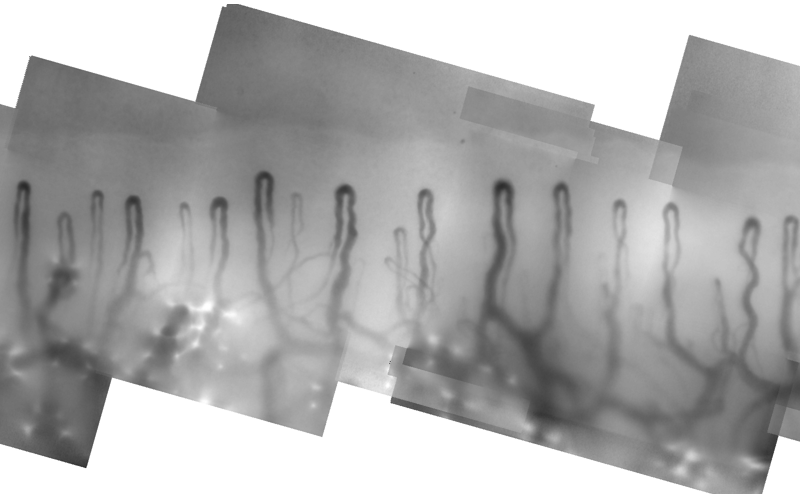
\includegraphics[width=0.48\columnwidth]{\figpath/nailfold_10598c_cropped}
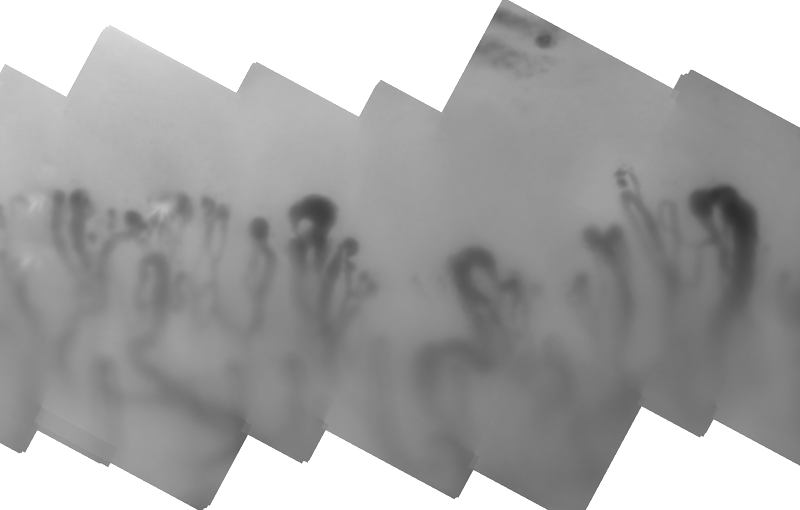
\includegraphics[width=0.48\columnwidth]{\figpath/nailfold_54611c_cropped} \\
\noalign{\smallskip}
\end{tabular}
%
\caption{Sections from two nailfold mosaics: one from a healthy control subject (left) and one from a patient with SSc (right) showing enlargement, distortion and irregular spacing of capillaries.}
\label{f:capillaroscopy}
\end{figure}
%
\section{Nailfold Capillaroscopy Data}
\label{s:data}
Our images were acquired by a capillaroscopy system in a tertiary referral centre for patients with SSc. Patients gave informed consent. High magnification, $768 \times 576$, 8-bit monochome pixel video frames were captured at a resolution of $1.25 \mu m$ per pixel. Images captured along the nailbed were registered and compounded into a single mosaic (similarly to~\cite{Anderson_etal_JRh05}) showing the whole nailfold (\fref{f:capillaroscopy}).

In normal subjects, capillary loops are all similar, arranged regularly and approximately vertical. Current clinical practice confines attention to the distal row of capillaries, whose apices lie on a smooth, approximately horizontal line near the top of the image. This pattern is disrupted in SSc by structural damage to the microvasculature (\fref{f:capillaroscopy}).

We have used a set of 990 mosaics, manually annotated as part of a separate clinical study, involving three subject groups: healthy controls (HC), subjects with PR, and patients with SSc. Each image was annotated independently by two expert observers, one of whom (Observer 1) was the same for every image, with the other drawn from a pool of experts. In each image, the observers attempted to mark the locations and apical widths of all distal capillaries. This is a challenging and subjective task for which perfect agreement is rare (see \sref{s:results}).

In a subset of 80 images, Observer 1 provided a precise demarcation of the inner and outer edges of the distal capillaries. Regions of interest around these capillaries were created, resulting in a set of 450 training RoIs with matching capillary masks, which we used for training learning algorithms (\sref{s:segmenting_vessels}, \sref{s:capillary_apexes}, \sref{s:distal_row}). The remaining images were split into a validation set of 456 images (104 HC, 83 PR, 269 SSc) used to locate capillaries and determine the distal row, and a test set of 455 images (104 HC, 83 PR, 268 SSc) used to evaluate performance (\sref{s:results}).
%
\section{Vessel Detection and Characterisation}
\label{s:segmenting_vessels}

Nailfold images are challenging -- capillaries are often very low contrast and of variable width ($10-300 \mu m$) and appearance, whilst significant artefacts can be present. Although previous work on automated capillaroscopy is limited, we can draw on the extensive literature on curvilinear structure detection in medical images (eg~\cite{Staal_etal_TMI04,Soares_etal_TMI06,Berks_etal_IPMI11}.  In particular, we adopt the well-established machine learning approach to predict, at each pixel, the probability that it belongs to a vessel (vesselness)~\cite{Soares_etal_TMI06}, and the local orientation and width~\cite{Berks_etal_IPMI11}. In the following sections we explain the features we used to describe local image structure, and the learning methods we used to obtain vesselness, orientation and width models.

\subsection{Image Features}
\label{s:image_features}
%Our choice of local structure representation is based on an extensive evaluation of alternatives, the details of which are beyond the scope of this paper.
To characterise local structure at each training pixel, we use a feature vector of responses to symmetric (even) and asymmetric (odd) filters across scale and orientation. Specifically, we use a steerable filter bank~\cite{Freeman_Adelson_TPAMI91} of directional second order derivatives of a Gaussian kernel~\cite{Staal_etal_TMI04} and their (approximate) Hilbert transforms so that responses at any orientation can be computed efficiently. From an initial scale $\sigma=1$ pixel we compute even and odd responses at six angles $\theta_i = \nicefrac{i\pi}{6}$ over five scales, in each case keeping $\sigma$ fixed whilst downsampling the image by a factor of $2$ in each direction (\ie~the coarsest scale is equivalent to $\sigma=16$ at the original image resolution). For the coarser scales, we use bilinear interpolation to approximate the responses at the finest scale. At each pixel the responses at that pixel, along with its 8-connected neighbours, are concatenated into a feature vector without further manipulation. These features are designed to accommodate the wide range in size, shape and orientation of imaged capillaries.

\subsection{Learning Vesselness, Orientation and Width Models}

We treat vessel detection as a supervised classification problem, and orientation and width prediction as regression problems, all based on the features outlined in the previous section. We have used Random Forests~\cite{Breiman_ML01}, due to their ease of training, flexibility, relative robustness to over-fitting and strong performance in comparable learning tasks, but we do not believe the choice of learning method is critical.

For training, we used the 80 fully annotated images described in \sref{s:data} each of which provides a binary vessel mask for training a vesselness classifier. To provide ground-truth for orientation and width regression, we skeletonised the binary masks, measured orientation and width at each centreline point, and propagated the measurements back to every point on the binary vessel mask using a simple nearest pixel interpolation. For orientation regression, we represented orientation as a unit vector in the complex plane, $t = \cos 2\theta + i\sin 2\theta$, doubling the angle $\theta$ to make orientation invariant to direction~\cite{Mardia_Jupp_00}, and avoiding �wraparound� problems that arise if angle is used directly.
%This permits a correct definition of variance for a set of orientations, the angular dispersion~\cite{Mardia_Jupp_00}, that is defined as the magnitude of the mean vector over the set \ie~$D = |(\sum{t_k})/N|$.
%This has a maximum of 1 when all $t_k$ are equal, and a minimum of 0 when orientations are distributed uniformly about the circle or when the sample consists of pairs exactly $180^\circ$ apart. Halving the inverse tangent of the mean vector returns the angular mean of the set in radians.

We trained three random forests (RFs), each containing 100 trees: one classifier on background versus labelled vessel pixels, and one regressor each for orientation and width. Although orientation and width are only defined for the vessel points, to ensure we generate unbiased, random predictions in the background of unseen images, we include background points with uniformly sampled random widths and orientations in training the regressors.

To make predictions in an unseen image we apply the separable basis filters, compute the interpolated, steered responses and extract feature vectors, before feeding the vectors through the trees in each forest and computing the mean, pooled over all leaf nodes, as the prediction output. For orientation, the unit vectors are converted back to radians. The result for each input image is a map of vesselness ($V_v$), orientation ($V_\theta$) and width ($V_w$) (\fref{f:detection_method}(a-b)). Note that predictions of width and orientation made in this manner are significantly more accurate than analytic estimates, and, by reusing the same features as extracted for $V_v$, requires minimal additional computation.

\section{Locating Candidate Capillary Apices}
\label{s:capillary_apexes}

The maps $V_v$, $V_\theta$ and $V_w$ provide an approximate segmentation of vessels and their low-level properties. However to extract meaningful measurements we need to detect and localise the apices of individual capillaries. Treating this as an object detection problem, we again adopt a learning approach in which each vessel pixel votes for the location of a nearby apex. Specifically, we use RF regression, trained using patches sampled near annotated capillary apices in the training data, to encode observed relationships between appearance and location~\cite{Criminisi_MICCAI11}.%,Roberts_etalMICCAI12

To train the RF, we thin $V_v$ by applying non-maximal suppression along the line normal to the estimated vessel orientation. We then extract $64 \times 64$ training patches, centred at local maxima in $V_v$ and scaled and rotated according to the estimated width and orientation. If a patch contains a marked apex and is also centred at a vessel pixel in the original training masks, we label the patch as positive and record the offset to the apex; otherwise, we label the patch as negative. %(Several positive patches are therefore associated with each apex.)
For each patch, a histogram of gradients (HoG) feature vector is formed by concatenating weighted histograms of gradient direction, computed for overlapping blocks in the patch~\cite{Dalal_Triggs_CVPR05}. A 100 tree RF classifier is then trained to distinguish between positive and negative patches, whilst a regression forest is trained to predict the offset associated with each positive patch.

For an unseen image, we extract a scale- and rotation-normalised patch about each local maximum in $V_v$ (\fref{f:detection_method}(b)) and pass these through the classification forest. The output labels at each leaf node are pooled and averaged, forming $\alpha(p)$, the probability that the patch contains an apex. The regression forest then predicts the offset to the nearest apex, and therefore the apex location in the image. A Gaussian kernel -- centred at the apex, scaled by $\sigma = V_w(a)$ and weighted by $\alpha(p)$ -- is added to a vote map of apex locations $A$. Here the classifier plays a crucial role in weighting the regressor votes, so that only patches in which an apex is visible significantly contribute to $A$.%\footnote{the scaling accounts for the fact that wider capillaries have a larger region in which an apex could reasonably be located}
The local maxima of $A$ are the candidate locations for capillary apices (\fref{f:detection_method}(c)).
%
\section{Refining Candidate Apices and Making Measurements}
\label{s:distal_row}
%
Given a set of candidate apex locations as training data, we can now train a new classifier that better discriminates between true apices and false positives, and between distal and non-distal apices. We do so in two ways:
first, we reclassify each candidate, now using patches located only at candidate apex locations;
second, we exploit the fact that capillaries should lie in a single, approximately horizontal line across the image.

To train the new classifier, we used candidate apices computed for the set of 441 validation images. Each candidate $(x_i,y_i)$ was labelled as positive only if it fell within a circle centred at a marked apex with diameter equal to the marked apical width. Of the 13,492 positive and 24,369 negative samples, the positive samples were further split into 9,735 distal and 3,757 non-distal capillaries. %\footnote{Where one observer marked a capillary as distal, and the other as non-distal, the label was randomly assigned to one of the two cases}}
A 100 tree RF classifier was trained as before, using HoG features from scale- and rotation-normalised patches extracted about each sampled candidate from the original image (rather than $V_v$). The outputs of the trees were pooled to give a single appearance score, $c_i \in [0, 1]$, for each candidate, allowing us to define each candidate as the tuple of its location and score, $(x_i,y_i,c_i)$.
%
\begin{figure}[t]
\centering
\begin{tabular}{@{}c c c@{}}
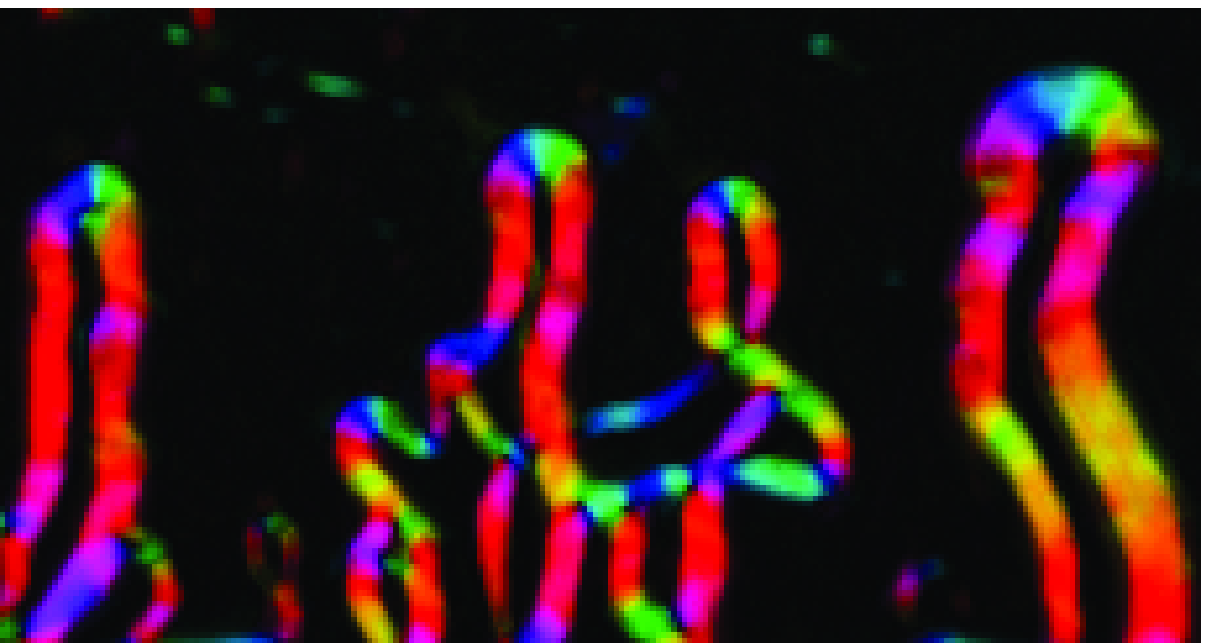
\includegraphics[width=0.31\columnwidth]{\figpath/02_orientation_prediction} &
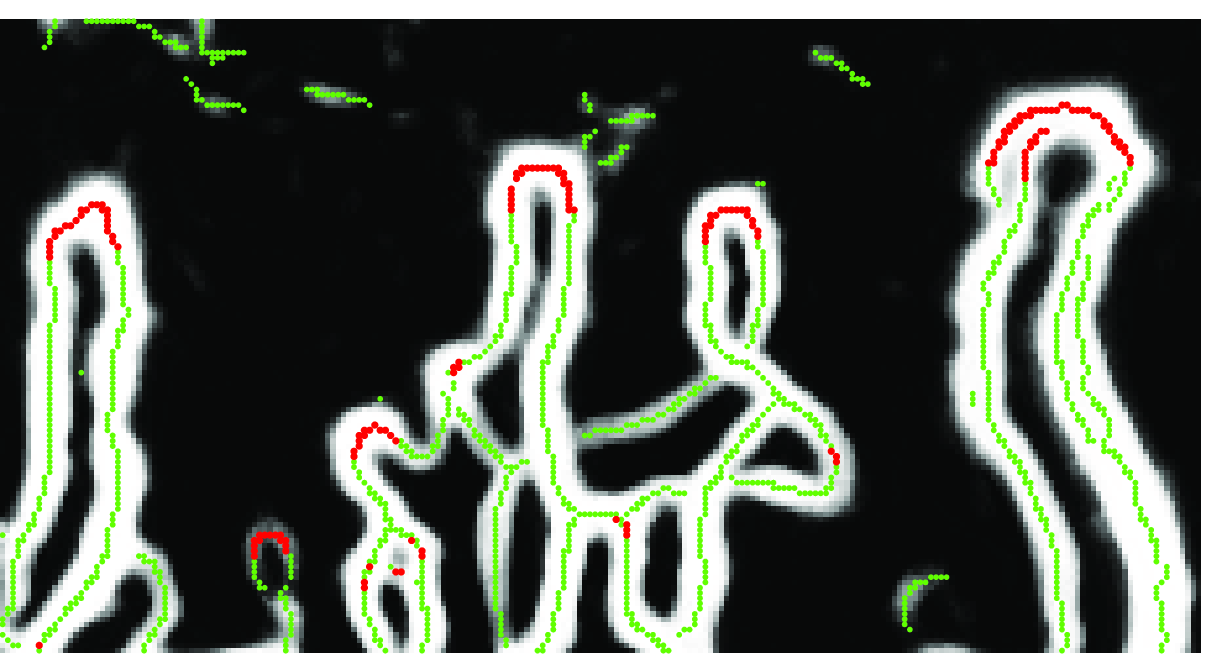
\includegraphics[width=0.31\columnwidth]{\figpath/01_vessel_prediction} &
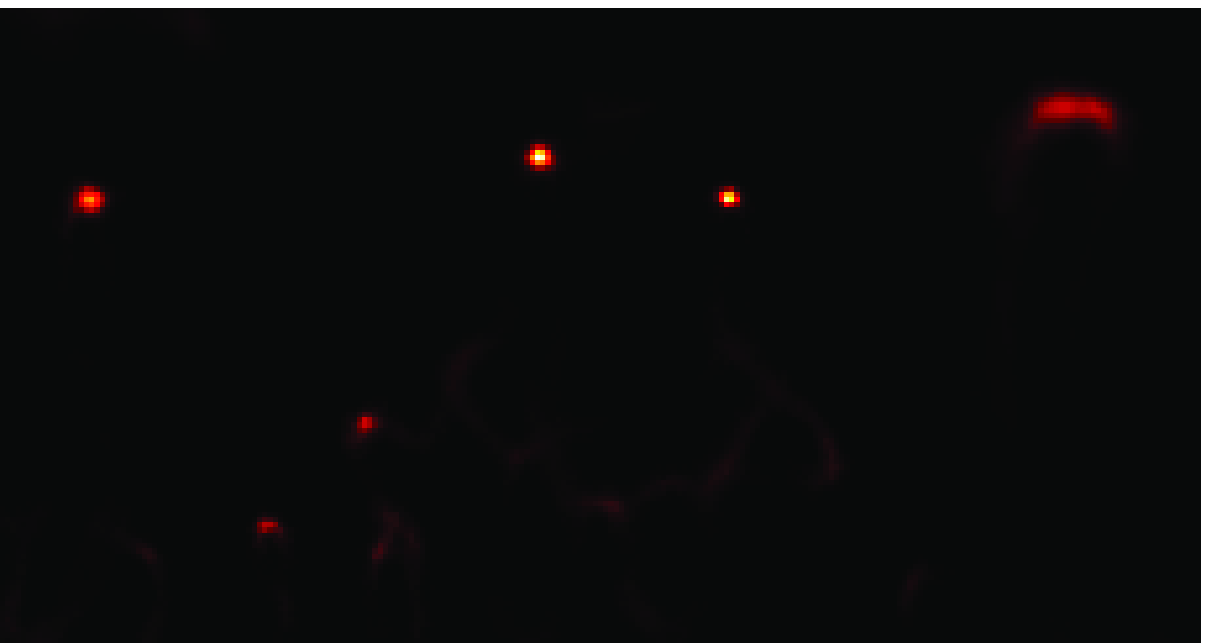
\includegraphics[width=0.31\columnwidth]{\figpath/03_apex_heat_map} \\
(a) & (b) & (c)\\
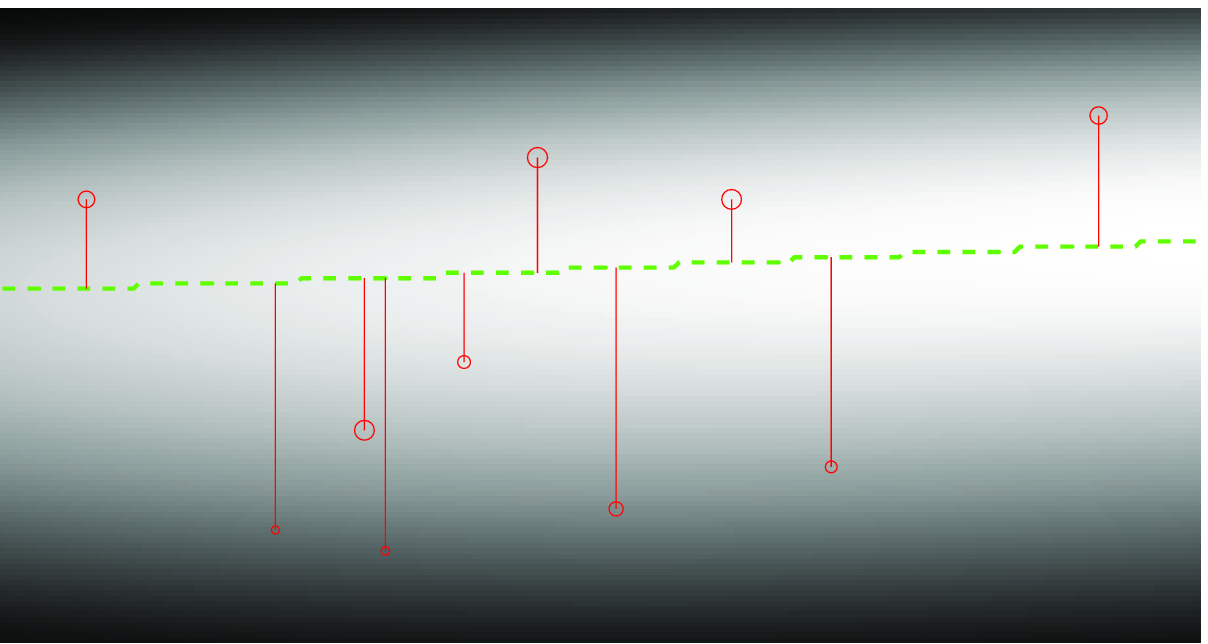
\includegraphics[width=0.31\columnwidth]{\figpath/04_apex_location_map} &
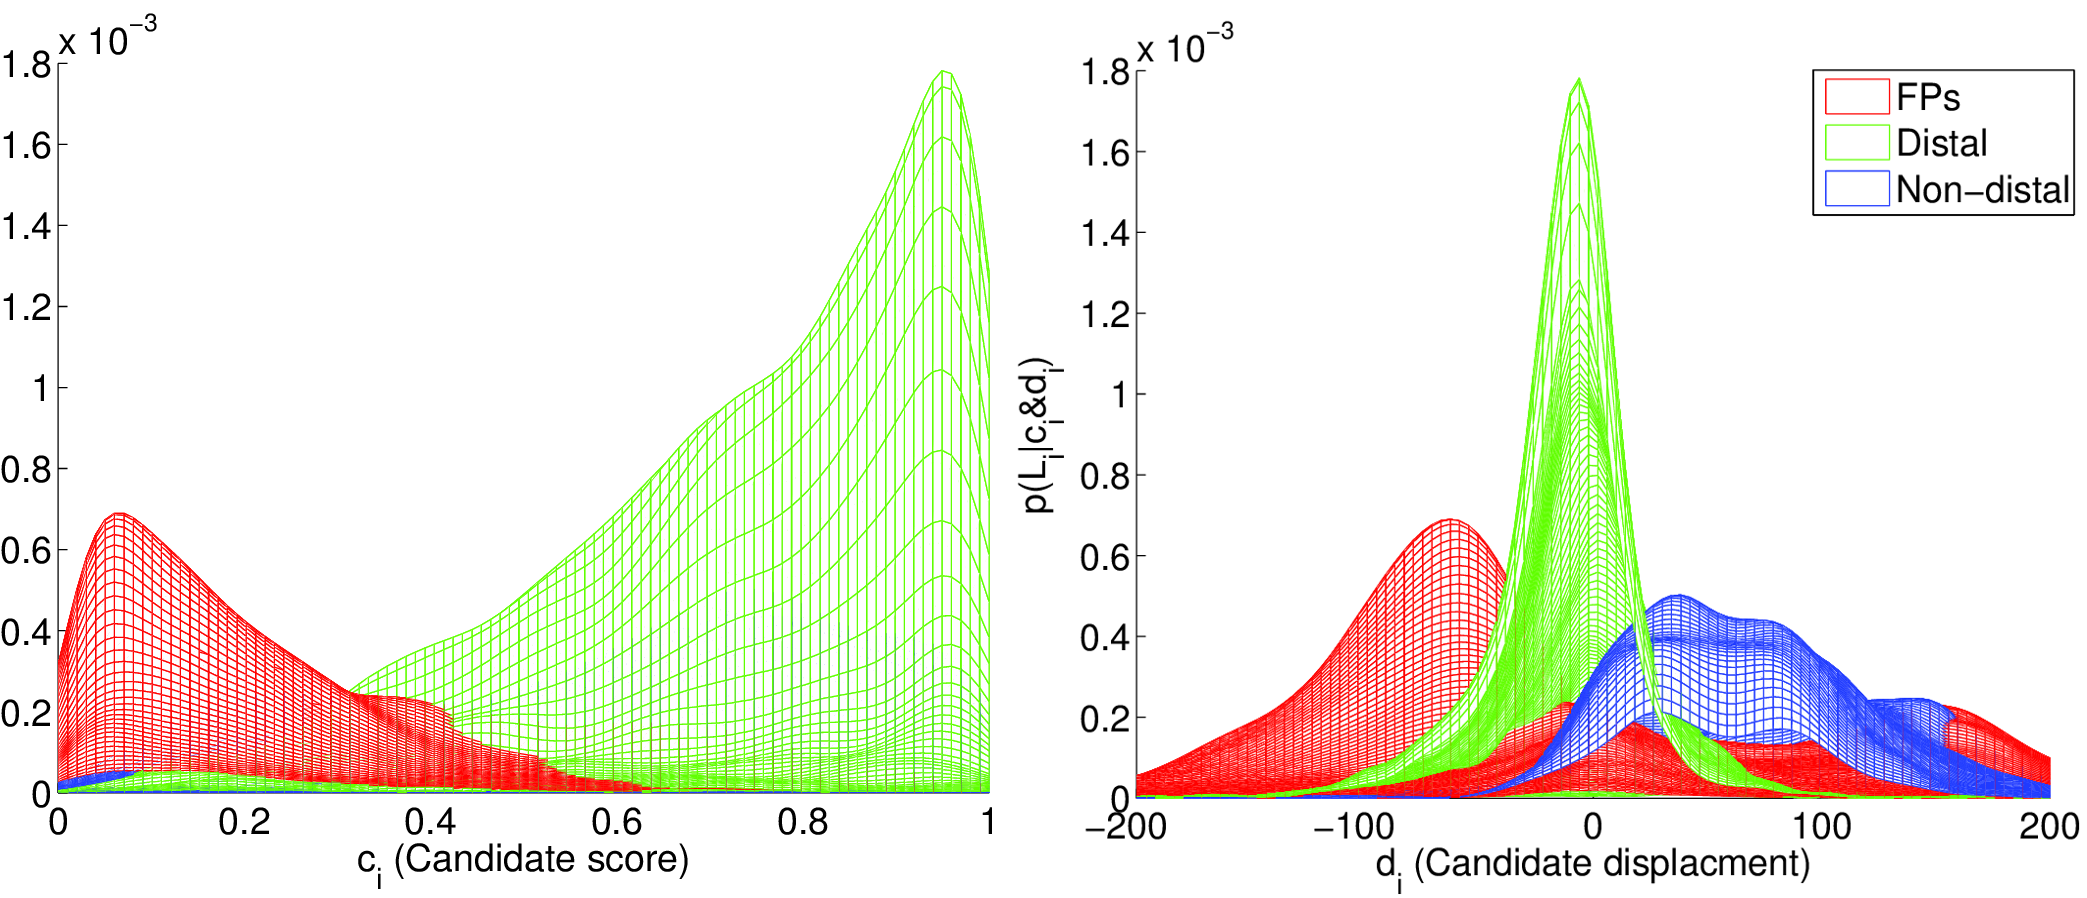
\includegraphics[width=0.31\columnwidth]{\figpath/05_conditional_pdfs} &
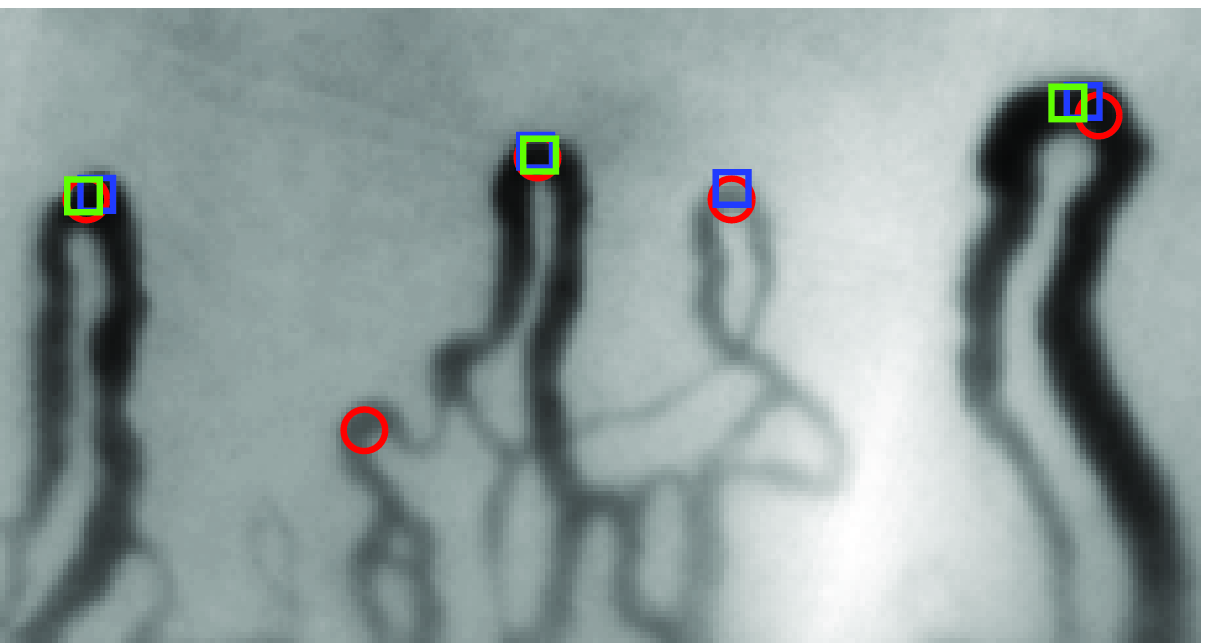
\includegraphics[width=0.31\columnwidth]{\figpath/00_nailfold} \\
(d) & (e) & (f)\\
\noalign{\smallskip}
\end{tabular}
%
\caption{Detecting nailfold capillaries %
(a) Estimated vessel orientation $V_\theta$, displayed using an hue/intensity color-map for angle/prediction confidence; %
(b) Vesselness $V_v$ with oriented local maxima marked by green dots. Red dots have $\alpha(q)>0.5$ and vote for apex locations; %
(c) Vote map $A$ of apex locations; %
(d) Estimated distal row (green line), from weighted kernel density of maxima in $A$. Candidate capillary locations are shown as red circles (scaled by candidate appearance score) with $y$ displacements to estimated distal line; %
(e) Mesh plots of the joint class conditional distribution over candidate displacement and appearance score, viewed from score axis (left) and displacement axis (right): false positves (red), distal capillaries (green), non-distal capillaries (blue); %
(f) Capillaries selected by our method (red circle) and experts observers (blue and green squares), solid markers show distal capillaries.
}
\label{f:detection_method}
\end{figure}
%
In addition to the final appearance score, the location of a candidate relative to the other candidates in any image can indicate its likelihood of being a distal row apex. Specifically, we assume the ideal distal row to be a smooth line running across the mosaic and passing through every true distal capillary apex. If we can estimate this line in an unseen image, we can use the vertical displacement of each candidate to the line to classify it as distal or nondistal.

To achieve this, we compute a density map of candidate locations by summing a Gaussian kernel centred at each discrete candidate location. Each kernel is weighted by the candidate's appearance score, $c_i$, so that strong candidates contribute more to the density. The density for each location in the mosaic can thus be computed as
%
\begin{equation}
D(u,v) = Z\sum\limits_{i=1}^N c_i\exp \left[ -\frac{(u-x_i)^2}{2{\sigma_x}^2}\right]\exp \left[ -\frac{(v-y_i)^2}{2{\sigma_y}^2}\right]
\label{e:kernel_estimate}
\end{equation}
where there are $N$ candidates in the image, $Z$ is a normalisation constant so that $D$ sums to unity, and $\sigma_x$, $\sigma_y$ are functions of the variances of $x_i$, $y_i$. Each apex's displacement from the distal row is then given by
%
\begin{equation}
d_i = y_i -  \operatorname*{arg\,max}_v D(x_i,v)
\label{e:candidate_displacment}
\end{equation}
%
Using the observers' annotations, each candidate $C_i=(x_i,y_i,c_i,d_i)$ in the validation images is assigned a label $L_i \in [1,2,3]$ for false positives, distal capillaries and non-distal capillaries respectively. \fref{f:detection_method}(e) shows a kernel estimate of the class-conditional probability density $P(c_i, d_i | L_i)$. The class priors for each label type $P(L_i)$ can be estimated empirically from the data, allowing Bayes' rule to be used to compute the class probability, $P(L_i | c_i, d_i)$, of each candidate, given its appearance score and displacement.

Each candidate is rejected, or labelled as either a distal or non-distal capillary. For each kept candidate $C_i$ we record its width $V_w(x_i,y_i)$, and use $V_\theta$ and $V_v$ to compute the entropy of an orientation histogram of pixels connected to $C_i$ as a measure of tortuosity. %(rather than selecting a hard threshold on connectivity, we weight the contribution of each pixel $p$ to the histogram by the largest threshold $\phi \in [0, 1]$ on $V_v$ such that $p$ and $C_i$ are connected)
Finally, we compute capillary density as the mean distance between the distal apexes.
%
\section{Results}
\label{s:results}
%
We applied our detection method ($O_3$) to the set of 455 test images, and compared the selected capillaries to the annotations of the two human observers ($O_1$ and $O_2$). In total, 15,391 capillaries were selected by at least one of the three observers. The results illustrate the difficulty of the task. For example, of the 7047 distal capillaries (DCs) marked by $O_1$, only 56\% were also marked by $O_2$, whilst 74\% were marked by the automated system ($O_3$). Defining true positives via consensus between the experts, of the 3913 DCs marked by both $O_1$ and $O_2$, 84\% were marked by $O_3$, which is a probably a workable performance level. Given the level of disagreement between the experts, false positives are even harder to assess. Of the 7913 DCs marked by $O_3$, 27\% were marked by neither $O_1$ nor $O_2$. On the other hand, of the 7047 DCs marked by $O_1$, 17\% were marked by neither $O_2$ nor $O_3$, and 44\% were not marked by $O_2$.

Overall, the results suggest similar performance between $O_1$, $O_2$ and $O_3$. To test this formally, we considered the capillaries (both distal and non-distal) selected by each observer as truth and assessed how well each of the two observers detected these capillaries. \tref{t:results} shows the precision, recall  and $F$-measure for each pair of observers. To test the labelling of capillaries as distal or non-distal, we considered all capillaries jointly selected by each pair of observers, and computed accuracy and Cohen's kappa statistic to quantify agreement. Accuracy and kappa statistics were not computed for capillary detection because there is no defined true negative class for the task (this is effectively the space of all images not containing a capillary). In addition to the pairwise tests, we computed equivalent values for the software versus the consensus of the two humans.

Standard errors for each value were computed from 1,000 bootstrap samples of the test images. For the $F$-measures and Cohen's kappa statistics we computed the difference between the agreement of $O_1$ and $O_2$ and the average of their individual agreement with $O_3$. $95\%$ confidence intervals of $(-7.01,-3.90)$ and $(-0.019,0.12)$ respectively, suggest there was no significant reduction between the software's performance and either human on the two tasks (if anything the software showed greater agreement to the humans individually than the humans did to each other on the detection task).
%
\begin{table}[tb]
\centering
%\small
\input{results_table.txt}
%
\caption{Pairwise agreement between observers. For each row $O_i$ v $O_j$ denotes the performance of observer $i$ using $j$ as ground truth. $O_1,O_2$ denotes consensus of the two human observers. Precision, recall and $F$-measures are given for vessel detection, classification accuracy and Cohen's Kappa statistic for labelling capillaries as distal or not.}
\label{t:results}
\end{table}
%
\begin{figure}[t]
\centering
\begin{tabular}{@{}c c c@{}}
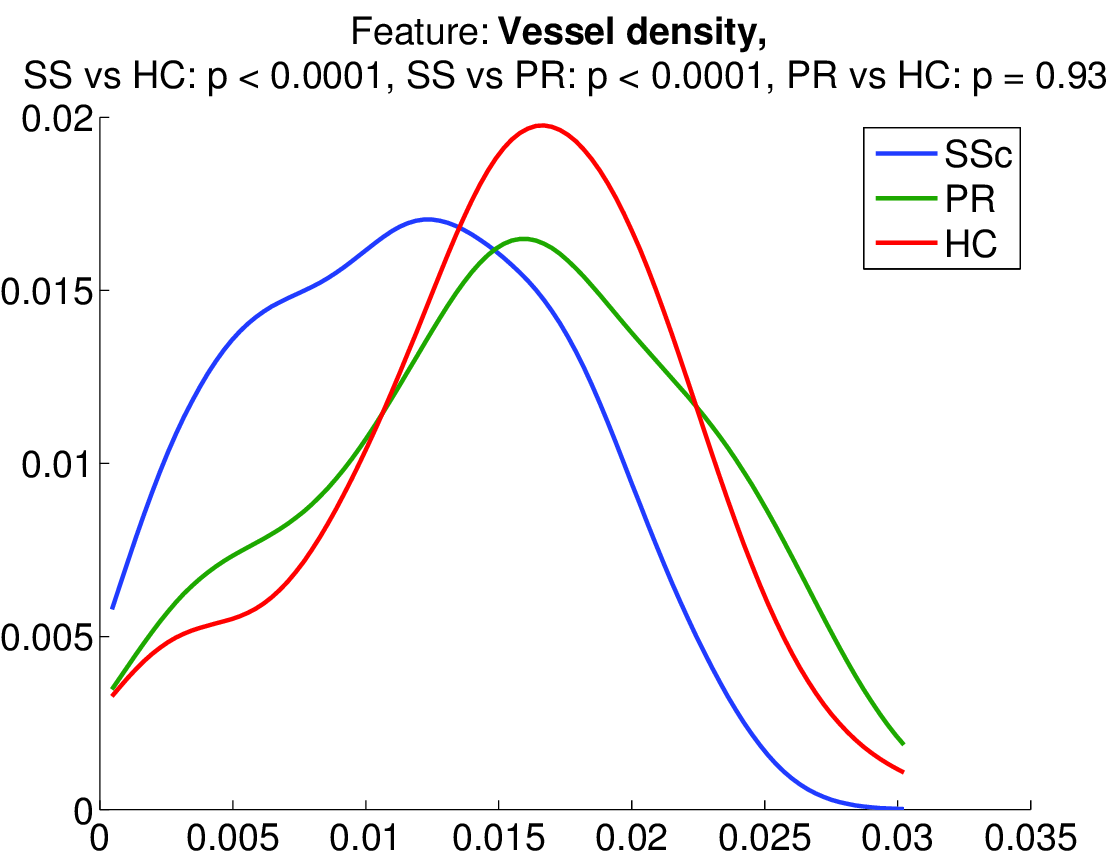
\includegraphics[width=0.31\columnwidth]{\figpath/vessel_density_pdf} &
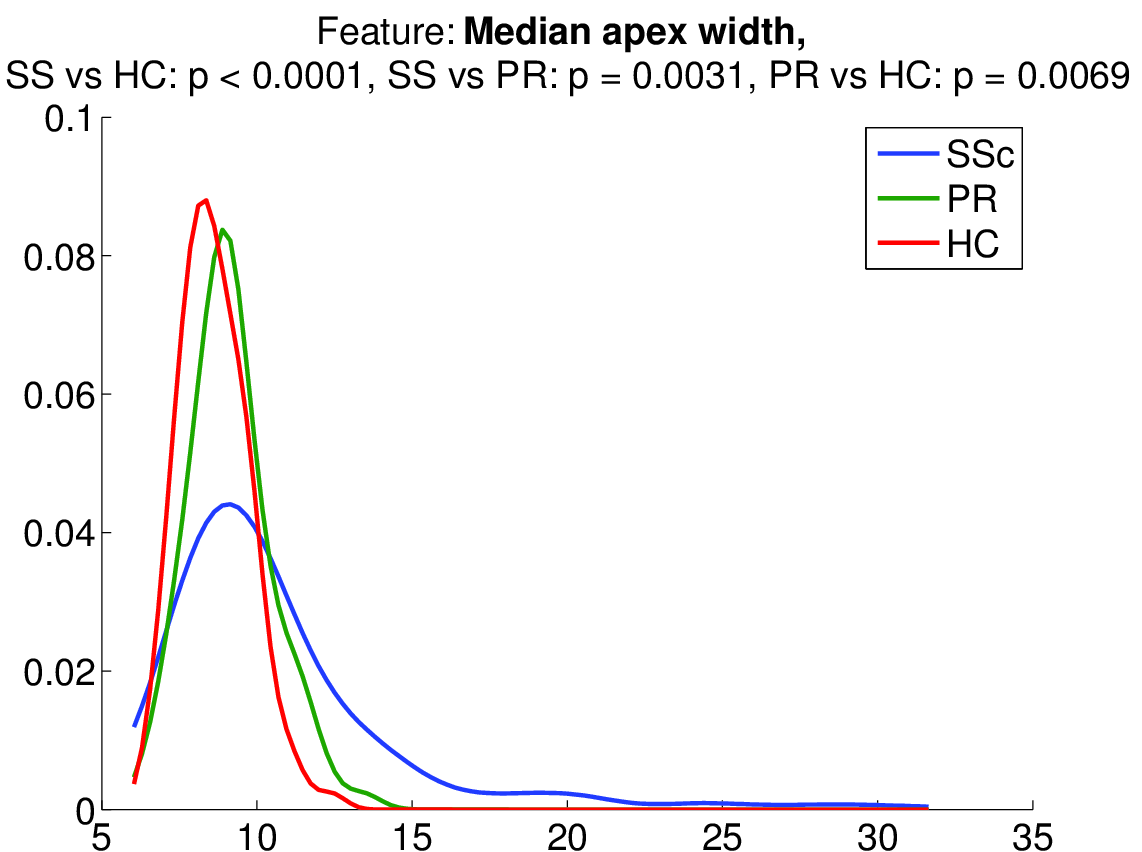
\includegraphics[width=0.31\columnwidth]{\figpath/median_apex_width_pdf} &
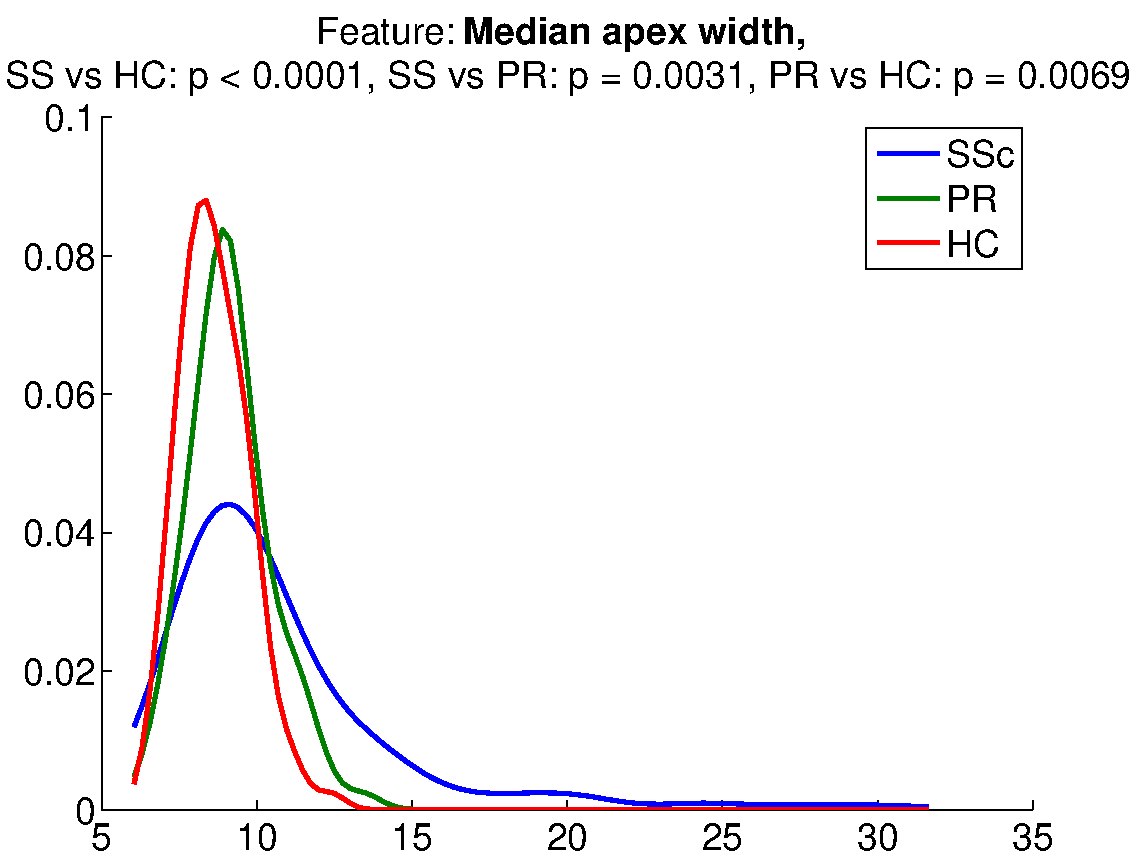
\includegraphics[width=0.31\columnwidth]{\figpath/median_orientation_entropy_pdf} \\
(a) & (b) & (c)\\
\noalign{\smallskip}
\end{tabular}
%
\caption{Distributions of capillary measurements by subject group: %
(a) Capillary density; %
(b) Median apical width; %
(c) Median capillary tortuosity.
}
\label{f:subject_apex_measures}
\end{figure}
%

%Visual inspection of the results suggest that many of the apparent false positives generated by the automated system are perfectly good DCs, and we are currently considering alternative evaluation strategies.

%To formally test the pairwise agreement between observers, we computed Cohen's kappa statistics. However to avoid under-estimating agreement, we must add a non-zero value for $O_1, O_2, O_3 = L_1$. This reflects the fact that wherever no observer marked a capillary, the observers have made an agreement that is otherwise not captured in our results. Defining $\kappa_z(i,j)$ as the kappa statistic between observers $i$ and $j$ for a `not marked' value of $z$, the limits as $z\rightarrow\infty$ can be analytically computed as $\kappa_\infty(1,2)=0.56$, $\kappa_\infty(1,3)=0.60$ and $\kappa_\infty(2,3)=0.62$. Empirically we found each limit was reached at $z\approx 10^5$, a rate equivalent to sampling $~10$ background patches per capillary.
%Bootstrap samples of the test images were used to compute a $95\%$ confidence-interval $CI = (-0.04,-0.07)$ for  $\kappa_\infty(1,2) - 0.5\left(\kappa_\infty(1,3)-\kappa_\infty(2,3)\right)$, implying that the automated software agrees at least as much with either expert as the two experts do with other.

Finally, we present initial results for disease status characterisation, based on the measurements extracted for the detected capillaries. Distributions of capillary measurements (capillary density, median width and median tortuosity) for the three groups HC (104 images), RP (83 images), and SSc (268 images) are shown in \fref{f:subject_apex_measures}. To test for differences between the distributions we used the non-parametric Wilcoxon rank sum test. Tests for all measurements between all groups showed significant differences at the 0.01 confidence level (at least), except for the comparison between RP and HC for vessel density -- an expected result given that we would not expect the RP group to show any signs of capillary loss.
%That difference between RP and HC can be observed for the width and tortuosity measurements (albeit with large overlaps in the group distributions), suggests our method may be sensitive to early changes in microvasculature that may be indicative of RP sufferers at risk of progressing to SSc.

\section{Conclusions}
\label{s:conclusions}
We have presented a fully automated system for measuring vessel morphology from nailfold capillaroscopy images. Evaluation on a large data set suggests that our system performs as well as experts in detecting vessels, and initial results for automated measurement suggest that we can detect significant differences between disease groups. Further work will involve refining apex detection, adding more sophisticated measurements, and combining measurements to make useful predictions for individuals.

\textbf{Acknowledgements.}
This work was funded by the Wellcome Trust. We are grateful to all the observers that annotated images used in the study.
%\end{document}

\bibliographystyle{splncs}
\bibliography{./bib/_aliases,./bib/miccai2014}

\end{document}
